\newpage
%\section*{Pregunta 4b}
\Large
b) El Problema de las Ocho Reinas consiste en acomodar ocho reinas de ajedrez en un tablero, sin que ninguna de éstas se ataque entre sí. Una reina, puede atacar (a) de forma vertical, (b) de forma horizontal y (c) en diagonal. Usando estas reglas, indicar si el siguiente tablero es una solución al problema de las ocho reinas.\\

\begin{figure}[h!]
\centering
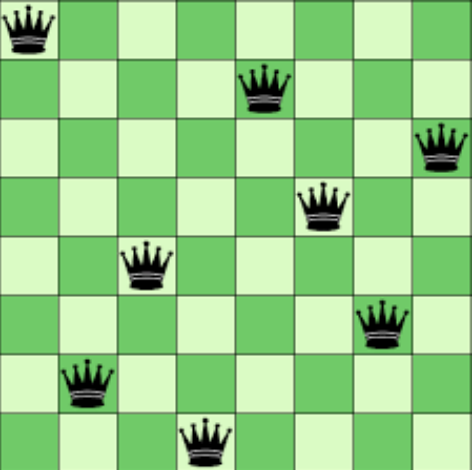
\includegraphics[scale=0.35]{Tablero.png}
\end{figure}
\large
Aqui pueden comenzar a poner sus respuestas.\\